\section{A bounded search finds every same-side route}\label{sec:connection}

\subsection{A rational honeycomb, with its elementary geometry}

For $h>0$, let the cell with axial indices $(i,j)\in\mathbb Z^2$
have center
\begin{equation}
 C_{ij}=h(3i,i+2j)
 \label{eq:centers}
\end{equation}
and, relative to that center, the six counterclockwise vertices
\begin{equation}
 h(2,0),\ h(1,1),\ h(-1,1),\
 h(-2,0),\ h(-1,-1),\ h(1,-1).
 \label{eq:hexvertices}
\end{equation}
Equivalently, the centered cell is
\[
 |y|\le h,\qquad |x+y|\le2h,\qquad |x-y|\le2h.
\]
The six neighbors, in the same edge order, have indices
\[
 (i+1,j),\ (i,j+1),\ (i-1,j+1),\
 (i-1,j),\ (i,j-1),\ (i+1,j-1).
\]

Here is a direct check that these cells tile the plane, rather than an
appeal to planar topology. Divide by $h$, fix $x=3i+t$ with
$0\le t\le3$, and inspect vertical slices.
For $0\le t\le1$, column $i$ has intervals of half-height one
centered at $i+2j$, and these abut and fill the vertical line.
For $1\le t\le2$, columns $i$ and $i+1$ have half-heights
$2-t$ and $t-1$, with centers alternating one unit apart.
The half-heights sum to one, so again the intervals abut exactly.
For $2\le t\le3$, column $i+1$ alone has half-height one.
This proves coverage and disjointness of cell interiors.
The neighbor list then verifies that precisely three cells and
three edges meet at a vertex, and no two edges cross except at
a shared endpoint.

Every cell lies within $2h$ of its center; every side has length at
most $2h$ in the maximum norm; and a link joining neighboring centers
has length at most $3h$. A center link crosses exactly its own common
side, at that side's midpoint, and otherwise lies in the interiors
of the two cells. In particular, a link between cells of the same
color avoids every edge separating different colors. These assertions
follow by substituting the six offsets in
\eqref{eq:hexvertices}. No separation property of a general polygon
is being used.

\subsection{Choosing the whole search region in advance}

Suppose the input clearances are $2^{-k_a}$ and $2^{-k_b}$. Set
\begin{equation}
 k=\max(k_a,k_b)+3,\qquad \delta=2^{-k},
 \qquad H=V(U(k+4))+10,\qquad h=2^{-H}.
 \label{eq:route-scale}
\end{equation}
Thus both input points have clearance at least $8\delta$.
Approximate them by rational points $a^*,b^*$ with errors at most
$\delta/16$. By the tiling property, select a cell containing each,
breaking ties by a fixed ordering, and let their centers be $a',b'$.
Then
\[
 \norm{a-a'},\norm{b-b'}\le\delta/16+2h<\delta/8.
\]
The two short endpoint connectors have clearance greater than
$7\delta$, and the center points have clearance greater than
$7\delta$. The original points and their centers have the same
curve bits.

Choose an integer $B\ge1$ larger by at least four than $R$ and than
the coordinate norms of $a^*,b^*$. Set
\begin{equation}
 L=\ceil{8B/h}+8,\qquad
 \mathcal C=\{(i,j): |i|\le L,\ |j|\le L\},\qquad
 M=(2L+1)^2.
 \label{eq:board}
\end{equation}
The selected cells of $a',b'$ are strictly inside this board.
For example $|3hi|\le B+2h$ bounds $|i|$, and
$|h(i+2j)|\le B+2h$ then bounds $|j|$, both far below $L-1$.
All searches for cells can therefore be full bounded scans of
$\mathcal C$.

Take the curve net at precision $H+4$. Its error is at most
$h/8$. For every neighboring-center link $S$ inside the board,
compute the rational distance estimate $D_S$ of
\eqref{eq:distance-net}, and make the decidable classification
\begin{equation}
 \begin{array}{ll}
 \text{safe},&D_S\ge 3h/2,\\
 \text{near},&D_S<3h/2.
 \end{array}
 \label{eq:linkcolors}
\end{equation}
The estimates prove
\begin{equation}
 \text{safe}\ \Longrightarrow\ \dist(S,\Gamma)\ge11h/8>h,
 \qquad
 \text{near}\ \Longrightarrow\ \dist(S,\Gamma)<13h/8<2h.
 \label{eq:linkcert}
\end{equation}
In the second case a finite minimizing sample and its rational
segment parameter explicitly witness the proximity; it is not an
unbounded existence test.

The outer ring of cells, $\max(|i|,|j|)=L$, is connected by
neighbor links: follow the four sides of the axial square using
the steps $(1,0)$ and $(0,1)$ and their negatives.
A center on this ring has norm at least $Lh$.
Indeed $|i|=L$ gives first-coordinate norm $3Lh$, while
$|j|=L$ and $|i|\le L$ give $|i+2j|h\ge Lh$.
Every ring link consequently lies outside the ball of radius
$(L-3)h$, which is larger than $R+2h$. The net test labels all
these links safe. Thus the outer ring has one reachability color.

\subsection{Flood fill and its finite boundary}

Start at the cell of $a'$ and mark all cells reachable by safe
links. This is a bounded algorithm: run reachability propagation
for $M$ rounds on the $M$-cell board, recording a parent at each
first discovery. A reached cell has a simple parent path with at
most $M-1$ edges. Conversely, deleting repeated vertices from a
finite walk produces such a simple walk, so no safe neighbor of
a reached cell remains unreached after $M$ rounds.

If the cell of $b'$ is reached, its parent path, together with the
two endpoint connectors, gives the answer. Its clearance is at
least $h$ and it has at most $M+1$ segments.

For the proof of success when bits agree, assume instead that the
cell of $b'$ is unreached. Color reached cells green and unreached
cells red. An edge between two cells of different colors is a
\emph{separating edge}. Its center link must be near, since a safe
link would make the reachability colors agree.

At a vertex with three incident cells, either all three colors
agree, giving no separating edges, or exactly one color differs,
giving exactly two separating edges. All outer-ring cells have
one color. The neighbor table shows that if a board vertex touches
an omitted cell, its incident included cells lie on this ring;
thus no separating edge can terminate at the outer boundary.
It follows that the finite separating graph has degree two
at every vertex it uses. Orient each separating edge with its
green cell on the left. The same three-cell check shows that
each used vertex has exactly one incoming and one outgoing edge.

Take a simple center-link path from the target cell to the source
cell, by changing the first axial coordinate and then the second.
Let $w$ be its last unreached center before its first reached
center $v$, and let $E$ be their shared side. It is a separating edge.
Starting with the oriented edge $E$, continue through the unique
outgoing separating edge at each vertex. There are at most $6M$ board edges.
The walk must repeat a vertex within that many steps.
The first repeated vertex is its initial vertex: otherwise the
unique predecessor at the earlier repeated vertex would already
have repeated. Therefore the walk gives a closed cycle $P$
with no repeated vertex before closure.
The tiling geometry makes it a simple polygonal cycle.

There can be several separating cycles on the board. We use only
the one through $E$; uniqueness of the entire boundary is neither
true in general nor needed.

Every point $z$ of a separating edge is within $3h$ of every
point of its crossed center link. Combine this finite geometric
bound with the near-link witness in \eqref{eq:linkcert}: $z$ is
within $5h$ of a known curve point. In particular, all vertices of
$P$ are within $16h$ of the curve, and its edges have length at
most $2h$. Lemma~\ref{lem:factor} applies with the scale
\eqref{eq:route-scale}.

\subsection{The local parity jump}

There is a safe center path from $a'$ to $v$, entirely through
green cells. There is a center path from $b'$ to $w$, the prefix
chosen above, entirely through red cells; its links need not be
safe. Both paths avoid every separating edge, since each of
their links joins cells of the same color. Consequently
\begin{equation}
 \parity(P,a')=\parity(P,v),\qquad
 \parity(P,b')=\parity(P,w).
 \label{eq:samecycle}
\end{equation}
We now prove the required change across $E$ by an elementary
deformation, rather than by invoking the polygonal Jordan theorem.

Translate $v$ to zero and write the side as $E=[p,q]$.
The parallelogram with successive vertices
\[
                  p,\ q,\ -p,\ -q
\]
is contained in the convex hexagon centered at $v$.
It contains $v$ strictly, while the neighboring center $w$ is
outside it. The link $vw$ meets its boundary exactly on $E$:
the link's first exit from the hexagon is at the midpoint of $E$,
and direct substitution of the six side types shows that this
is also its exit from the parallelogram.
Call this parallelogram boundary $Q$.

Replace the side $E$ in $P$ by the other three sides of $Q$,
obtaining a closed walk $P'$. It need not be simple.
The original center link met $P$ only on $E$, and it meets none
of the three replacement sides. Thus $P'$ avoids $vw$ and
\[
                  \parity(P',v)=\parity(P',w).
\]
As chains modulo two, $P'=P+Q$. The convex calculation in
Lemma~\ref{lem:triangle} gives $\parity(Q,v)=1$ and
$\parity(Q,w)=0$. Therefore
\begin{equation}
                  \parity(P,v)\xor\parity(P,w)=1.
 \label{eq:jump}
\end{equation}
All the avoidances just used concern finite rational segments.
Their positive clearances can either be read off the six cell
configurations or computed as finite rational minima.

\begin{theorem}[Connection alternative]\label{thm:connection}
For any two off-curve points, the bounded construction above
returns a route with clearance at least $h$, or proves that
their curve bits differ. In particular it always returns a
route when the bits agree.
\end{theorem}

\begin{proof}
The only unresolved case is an unreached target. In that case
\eqref{eq:samecycle}, \eqref{eq:jump}, and
Lemma~\ref{lem:factor}, applied to the two center points, give
\[
 1=\parity(P,a')\xor\parity(P,b')
   =m_P\bigl(b_\Gamma(a')\xor b_\Gamma(b')\bigr).
\]
In the two-element field, a product is one only when both
factors are one. The endpoint bits therefore differ, and
they are the same as the original input bits.
If the original bits agree, the unreached branch contradicts
this finite bit equality; the reached branch supplies the
route. This is elimination of one outcome of a decidable
finite calculation, valid in intuitionistic logic.
\end{proof}

\begin{figure}[tb]
\centering
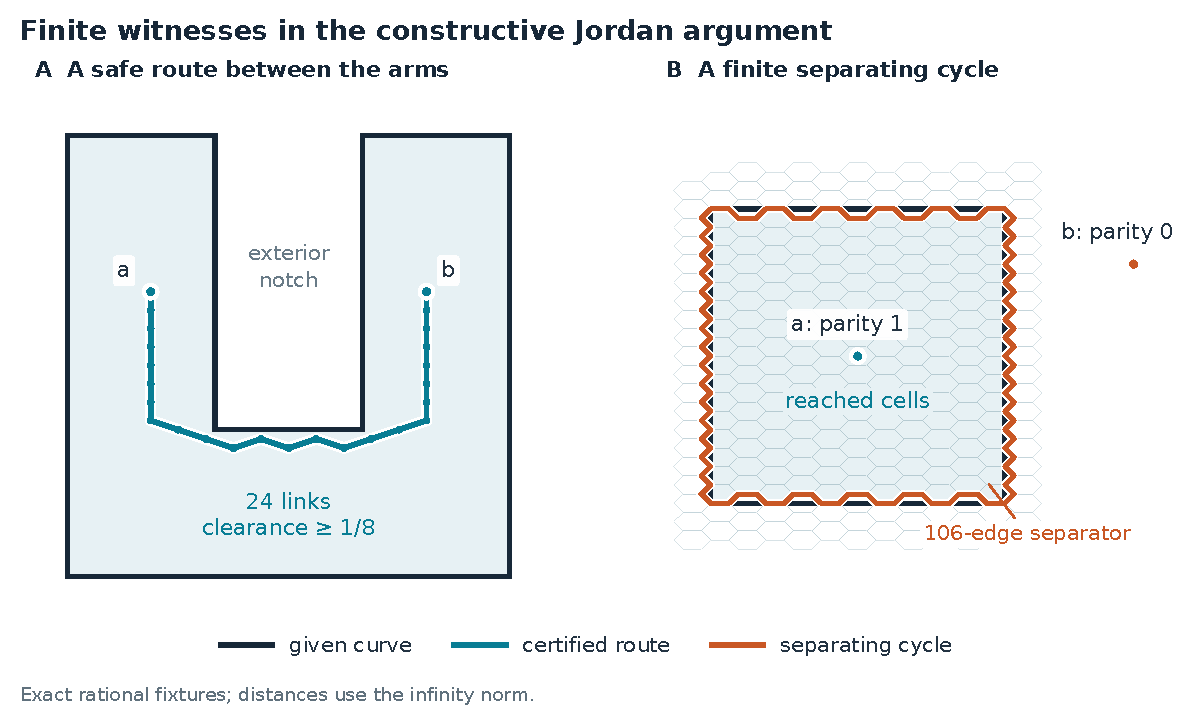
\includegraphics[width=\textwidth]{figures/finite_routes.pdf}
\caption{Exact finite examples from the accompanying kernel. Left:
a safe honeycomb route joins the two arms of a concave polygon;
its maximum-norm clearance is $1/8$. Right: flooding from a square's
interior leaves an exterior target unreached and produces a separating
cycle. These examples illustrate the finite constructions; the proof
above applies to the general named curve by the certified net test.}
\label{fig:routes}
\end{figure}
